\chapter{Introduction}\label{sec:intro}
\begin{flushright}{\slshape    
The most important contribution of management in the 20th century\\
was to increase manual worker productivity fifty-fold.\\
The most important contribution of management in the 21st century\\
will be to increase knowledge worker productivity\\
— hopefully by the same percentage} \\ \medskip
--- Peter F. Drucker~\cite{drucker1999}
\end{flushright}

\noindent When Drucker realized that the automation of manual labour was progressing faster than that of knowledge work, he voiced the words above at the end of the $20^{th}$ century in 1999. Now, 20 years later, the automation of semi-structured knowledge work has picked up speed due to the general adaption of tracking systems and the proliferation of machine learning techniques around business processes~\cite{boehmer2018probability, klinkmuller2018reliablemonitoring}.
In this thesis, we apply machine learning to business process log data to predict the next activity in a running business process, given its history. This chapter gives motivating reasons to do so in \autoref{sec:intro:motivation}, and highlights the resulting contribution to current research in \autoref{sec:intro:contribution}. The chapter ends in \autoref{sec:intro:outline} with a description of the thesis outline.

\section{Motivation} \label{sec:intro:motivation}
Automation of work is a phenomenon that has occurred in the past with manual labor, and is spreading into other types of work today, namely knowledge work. Both types of work differ strongly, as described in the following:

The course of manual labour is determined by physical laws, is often very structured, and thus offers great potential for easy automation - like work at an assembly line. Knowledge work on the other hand requires workers to "think for a living", and is strongly shaped by the individuality of the thoughts and habits of each knowledge worker~\cite{drucker1999}. As each worker has a different knowledge background, and uses information differently, this type of work is very flexible and often no process is executed exactly the same~\cite{hewelt2016}. A popular example for knowledge work are insurance claims, handled by several employees. Each claim requires a different course of action, since the information contained in each case differs.\\
%If the case takes an unwanted course, a possibility for early intervention is useful.\\

Forecasting the course of a running process, henceforth referred to as case or process instance, is of interest to both types of work. Manual labour is often dominated by questions of time and outcome~\cite{rogge2013} because the course of work is clear - natural interests in a world of distributed supply chains and just-in-time production~\cite{web:economist:jit}. The course of work itself is an object of interest in the case of unstructured knowledge work~\cite{francescomarino2015}. Knowing about the development of a case presents workers with an opportunity to intervene if it were to progress in an unwanted fashion.

In the 20 years since Drucker's statement, the analog tools of knowledge workers have evolved into a plethora of digital systems and applications. These knowledge repositories and assistance systems for knowledge workers help make their decisions more informed and faster. In doing so, these systems also track work progress, resulting in logs which document the trace of a case.\\

These logs are a valuable source of data as they can reveal best practices that knowledge workers use in certain situations. If this data were processed, such best practices could be recommended by an auxiliary system. These knowledge worker assistance systems have been called for multiple times in recent literature reviews~\cite{hauder2014, francescomarino2018}, but have only been implemented prototypically until now. The following chapter lays out the exact challenges for these systems that we have identified in the literature and how we tackle them. Putting the ability to forecast a process development into perspective, it is possible to see that it is a step toward process automation, because then the machine knows the \textit{what} and is only missing the \textit{how}.

\section{Contribution}\label{sec:intro:contribution}
One of the challenges that lie in the way of creating assistance systems is the task of anticipating the development of a case, especially that of the next activity. In this area, we make a contribution to ongoing research by applying predictive analytics using neural networks on process execution logs. Through the execution history of an incomplete case, the prediction of its next activity is then made possible, also illustrated in \autoref{fig:next-activity-prediction}. This next step could then be processed further by the aforementioned assistance system, e.g. to propose an intervention if a case takes an unwanted course. The application of Predictive Analytics on business processes is fairly new, and is commonly referred to as Predictive Process Monitoring.\\

\begin{figure}
    \centering
    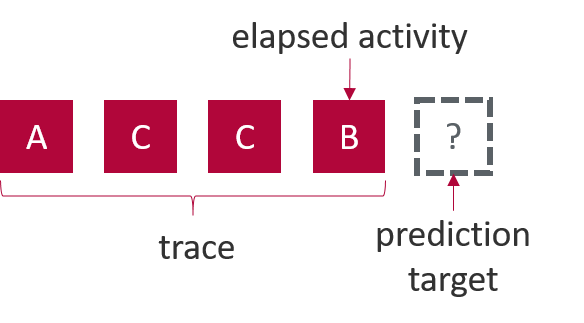
\includegraphics[width=\textwidth]{gfx/next-activity.png}
    \caption{Predicting the next activity, TODO: STOLEN GFX REPLACE OR ADAPT AND CITE?}
    \label{fig:next-activity-prediction}
\end{figure}

While working with the literature on Predictive Process Monitoring, we realized that the current research in this young domain can be improved in the following three areas:

\begin{enumerate}
    \item Comparability: Published approaches are not easily comparable, as their performance measures are based on different datasets. There is only a tendency to make use of the datasets of the Business Process Intelligence Challenge (BPIC)~\cite{BPIC2011, BPIC2012, BPIC2017}.
    \item Reproducibility: Divergent approaches to train the prediction models and low technical depth make it hard to reproduce the published results. Furthermore, some prediction approaches are not focused on a single case but whole event streams without specific regard to a case~\cite{evermann2016, schoenig2018}.
    \item NLP-Influence: The trace of a case is essentially a sequence, but little inspiration has been taken from Natural Language Processing (NLP), where sequence prediction is common~\cite{shibata2016bipartite}.
\end{enumerate}

We want to add value in these three areas by modifying a successful sequence prediction approach from a NLP competition and applying it on business process log data. To allow for a direct comparison, we test it on the datasets of BPIC 2011, 2012, and 2017, and compare it to two implementations that we reverse-engineered from the following publications:
\todo[inline]{adapt BPIC years}

\begin{enumerate}
    \item \textit{A Deep Learning Approach for Predicting Process Behaviour at Runtime} by Evermann et al.~\cite{evermann2016}
    \item\textit{Deep Learning Process Prediction with Discrete and Continuous Data Features} by Schönig et al.~\cite{schoenig2018}.
\end{enumerate}

Over the course of reverse-engineering the comparison models and the subsequent evaluation, widely divergent understandings and approaches with regard to the batch structure of sequential training data input for neural networks were uncovered. To contribute to a better understanding in this area, a comparison of the perceived possibilities was incorporated into the evaluation of the models. By using different datasets with very different trace characteristics we can infer a suggestion on which method to use for which flavor of case log.
\todo[inline]{what to do here?}

Furthermore we realized that typical model evaluations only measure total accuracy, while we believe that a stable accuracy across the whole execution of the process is key for putting trust into the model~\cite{francescomarino2015, boehmer2018probability}. These measurements form the second part of our evaluation. In a third part, we investigate the resource consumption.

Finally, we attempt a first step toward streamlining the comparison of process prediction models. Currently, implementations and datasets vary widely between publications, making comparability an issue. With the learnings about the training data formats in mind, we propose a simple process prediction comparison framework that helped us conduct our measurements, and which can be easily expanded with other models and data formatting approaches.

\section{Thesis Outline}\label{sec:intro:outline}
A preliminary definition of Predictive Process Monitoring and how it differs from Process Mining is delivered in \autoref{chap:background}. Furthermore this chapter provides information on Predictive Model Development as well as details on the inner workings of the used type of neural networks.

Then, \autoref{chap:related-work} gives an overview of current approaches to the prediction task at hand, highlighting the achievements and technicalities of each publication. Furthermore it presents work that was done on the problem of sequence prediction in the field of Natural Language Processing (NLP). For each publication used as comparison, the work is presented with implementation details and performance measures.

In \autoref{chap:taking-inspiration}, we show how sequences relate to business processes. Then, we go on to adapt a winning approach from an NLP sequence prediction competition for Predictive Process Monitoring, and enhance it with different features. In \autoref{chap:training-framework}, we describe an important technicality that we encountered during the implementation of the predictive models. We expand the technical overhead from this detail into a simple training framework that makes it possible to compare all models and batch strategies side-by-side on all datasets. We believe that it makes it easier for future researchers to try out custom models and reproduce others.

In \autoref{chap:evaluation} we bring both of the aforementioned contributions together and present the implementation and evaluation of these. We end the chapter with the insights gained from the subsequent measurements. As described in the previous section, we not only focus on total model accuracy, but also stability of the predictions as a case progresses and more history becomes available.

The thesis ends with \autoref{chap:conclusion}, which summarizes the findings and the accomplishments of this thesis. Furthermore we give pointers with which to extend this work and carry Predictive Process Monitoring forward.